\usepackage{luatexja}
\usepackage[hiragino-pron, nfssonly, deluxe, expert]{luatexja-preset}
\usepackage{pgfpages}
\usepackage{fontspec}
\usepackage{epigraph}
\usepackage{etoolbox}
\usepackage{tikz}
\usepackage{framed}
\usepackage{mathtools}
\usepackage{listings}
\usepackage{libertine}
\usepackage{bxcoloremoji}
\usepackage{xcolor}
\usepackage{multirow}
\usepackage{diagbox}
\usepackage{caption}
\usepackage{tikz-qtree}

\definecolor{links}{HTML}{2A1B81}
\hypersetup{colorlinks,linkcolor=,urlcolor=links}

\usetheme{Boadilla}
\usecolortheme{seahorse}
% \usefonttheme{serif}

\setbeamercolor{page number in head/foot}{bg=blue!10}
\makeatother
\setbeamertemplate{footline}
{
  \leavevmode%
  \hbox{%
    \begin{beamercolorbox}[wd=.4\paperwidth,ht=2.25ex,dp=1ex,center]{author in head/foot}%
      \usebeamerfont{author in head/foot}\insertshortauthor\hspace*{1ex}(\insertshortinstitute)
    \end{beamercolorbox}%
    \begin{beamercolorbox}[wd=.3\paperwidth,ht=2.25ex,dp=1ex,center]{title in head/foot}%
      \usebeamerfont{title in head/foot}\insertshorttitle
    \end{beamercolorbox}%
    \begin{beamercolorbox}[wd=.2\paperwidth,ht=2.25ex,dp=1ex,center]{date in head/foot}%
      \insertshortdate
    \end{beamercolorbox}%
    \begin{beamercolorbox}[wd=.1\paperwidth,ht=2.25ex,dp=1ex,center]{page number in head/foot}%
      \insertframenumber{} / \inserttotalframenumber\hspace*{1ex}
    \end{beamercolorbox}}%
  \vskip0pt%
}
\makeatletter

\beamertemplatenavigationsymbolsempty

\setbeamertemplate{bibliography item}{\insertbiblabel}
\setbeamersize{description width=1cm}
\setbeamertemplate{items}[circle]
\setbeamertemplate{section in toc}[circle]
\setbeamertemplate{subsection in toc}{%
  \leavevmode\leftskip=2em
  {%
    \usebeamerfont*{itemize item}%
    \usebeamercolor{subsection number projected}%
    \color{bg}%
    \raise1.25pt\hbox{\donotcoloroutermaths$\bullet$}}%
  \hskip1.5ex\inserttocsubsection\par}
\setbeamercolor{title}{bg=white}
\setbeamertemplate{title page}
{%
  \vbox{}
  \vfill
  \begingroup
    \centering
    \hrulefill
    \vskip1em\par
    \begin{beamercolorbox}[sep=8pt,center,shadow=false,rounded=true]{title}
      \usebeamerfont{title}\inserttitle\par%
      \ifx\insertsubtitle\@empty%
      \else%
        \vskip0.25em%
        {\usebeamerfont{subtitle}\usebeamercolor[fg]{subtitle}\insertsubtitle\par}%
      \fi%     
    \end{beamercolorbox}%
    \hrulefill
    \vskip1em\par
    \begin{beamercolorbox}[sep=8pt,center,shadow=false,rounded=true]{author}
      \usebeamerfont{author}\insertauthor
    \end{beamercolorbox}
    \begin{beamercolorbox}[sep=8pt,center,shadow=false,rounded=true]{institute}
      \usebeamerfont{institute}\insertinstitute
    \end{beamercolorbox}
    \begin{beamercolorbox}[sep=8pt,center,shadow=false,rounded=true]{date}
      \usebeamerfont{date}\insertdate
    \end{beamercolorbox}\vskip0.5em
    {\usebeamercolor[fg]{titlegraphic}\inserttitlegraphic\par}
  \endgroup
  \vfill
}
\setbeamertemplate{blocks}[rounded][shadow=false]
\setbeamertemplate{note page}{\pagecolor{yellow!5}\insertnote}


% ============ ここを消すとNote消える ================
% \mode<handout>{%
%   \setbeameroption{show notes on second screen=right}%
% }
% ============ ここを消すとNote消える ================


\renewcommand{\kanjifamilydefault}{\gtdefault}

\resetcounteronoverlays{lstlisting}
\definecolor{bluegray}{rgb}{0.4, 0.6, 0.8}
\DeclareCaptionFormat{listing}{{\color{bluegray}\lstlistingname}#2#3}
\captionsetup[lstlisting]{format=listing, font={footnotesize}}

\setmonofont[Ligatures=TeX]{CMU Typewriter Text}

\newcommand{\xcolon}{:}
\newcommand{\Fujitask}{{\rmfamily\bfseries Fujitask}}

\title[Fujitask meets Extensible Effects]{%
  {\bfseries\rmfamily\mcfamily\huge\scshape
    \Fujitask \\
    meets\\
    Extensible Effects%
  }%
}
\author[Hikaru Yoshimura]{%
  Hikaru \textsc{Yoshimura}(吉村 優)
}
\date[ScalaMatsuri, June 209 2019]{%
  \href{https://www.tryswift.co/events/2019/tokyo/en/}{ScalaMatsuri on \oldstylenums{June 29, 2019}} \\
  {\scriptsize (\href{https://github.com/y-yu/fujitask-eff-slide}{\texttt{y-yu/fujitask-eff-slide@\GITAbrHash}})}%
}
\institute[Recruit Markting Partners Co., Ltd.]{%
  Recruit Markting Partners Co., Ltd.\\
  \href{mailto:yyu@mental.poker}{yyu@mental.poker}
}

\newfontfamily\quotefont[Ligatures=TeX]{Linux Libertine O} % selects Libertine as the quote font

\newcommand*\quotesize{60} % if quote size changes, need a way to make shifts relative
% Make commands for the quotes
\newcommand*{\openquote}
   {\tikz[remember picture,overlay,xshift=-4ex,yshift=-2.5ex]
   \node (OQ) {\quotefont\fontsize{\quotesize}{\quotesize}\selectfont``};\kern0pt}

\newcommand*{\closequote}[1]
  {\tikz[remember picture,overlay,xshift=1.5ex,yshift={#1}]
   \node (CQ) {\quotefont\fontsize{\quotesize}{\quotesize}\selectfont''};}

\newcommand*\shadedauthorformat{\emph} % define format for the author argument

% Now a command to allow left, right and centre alignment of the author
\newcommand*\authoralign[1]{%
  \if#1l
    \def\authorfill{}\def\quotefill{\hfill}
  \else
    \if#1r
      \def\authorfill{\hfill}\def\quotefill{}
    \else
      \if#1c
        \gdef\authorfill{\hfill}\def\quotefill{\hfill}
      \else\typeout{Invalid option}
      \fi
    \fi
  \fi}
% wrap everything in its own environment which takes one argument (author) and one optional argument
% specifying the alignment [l, r or c]
%
\newenvironment{shadequote}[2][l]%
{\authoralign{#1}
\ifblank{#2}
   {\def\shadequoteauthor{}\def\yshift{-2ex}\def\quotefill{\hfill}}
   {\def\shadequoteauthor{\par\authorfill\shadedauthorformat{#2}}\def\yshift{2ex}}
\begin{quote}\normalfont\openquote}
{\shadequoteauthor\quotefill\closequote{\yshift}\end{quote}}

\makeatletter
\def\@fnsymbol#1{\ensuremath{\ifcase#1\or *\or \dagger\or \ddagger\or
   \mathsection\or \mathparagraph\or \|\or **\or \dagger\dagger
   \or \ddagger\ddagger \else\@ctrerr\fi}}
\makeatother

\renewcommand{\thefootnote}{\fnsymbol{footnote}}

\usetikzlibrary{shapes.callouts} 

\pgfkeys{%
    /calloutquote/.cd,
    width/.code                   =  {\def\calloutquotewidth{#1}},
    position/.code                =  {\def\calloutquotepos{#1}}, 
    author/.code                  =  {\def\calloutquoteauthor{#1}},
    at/.code                      =  {\def\calloutquoteat{#1}},
    /calloutquote/.unknown/.code   =  {\let\searchname=\pgfkeyscurrentname
                                 \pgfkeysalso{\searchname/.try=#1,                                
    /tikz/\searchname/.retry=#1},\pgfkeysalso{\searchname/.try=#1,
                                  /pgf/\searchname/.retry=#1}}
                            }  


\newcommand\calloutquote[2][]{%
       \pgfkeys{/calloutquote/.cd,
         width               = 5cm,
         position            = {(0,-1)},
         at                  = {(0,0)},
         author              = {}}
  \pgfqkeys{/calloutquote}{#1}                   
  \node [rectangle callout,callout relative pointer={\calloutquotepos},text width=\calloutquotewidth,/calloutquote/.cd,
     #1] (tmpcall) at \calloutquoteat {\hfil#2\hfil};
  \node at (tmpcall.pointer){\calloutquoteauthor};    
}

\newfontfamily\listingfont{Menlo}
\definecolor{dkgreen}{rgb}{0,0.6,0}
\definecolor{gray}{rgb}{0.5,0.5,0.5}
\definecolor{mauve}{rgb}{0.58,0,0.82}

\makeatletter
\lst@CCPutMacro\lst@ProcessOther {"2D}{\lst@ttfamily{-{}}{-{}}}
\@empty\z@\@empty
\makeatother

\lstdefinestyle{csharp}{
  numbers=left,
  language=[Sharp]C
}

\lstdefinestyle{cil}{
  numbers=left,
  language=CIL
}

\lstdefinestyle{plain}{
  numbers=left,
  language=
}

\lstdefinestyle{sh}{
  numbers=left,
  language=sh
}

\lstdefinestyle{c}{
  numbers=left,
  language=C
}

\lstdefinestyle{python}{
  numbers=left,
  language=Python
}

\lstdefinestyle{asm-x86}{
  numbers=left
}

\lstdefinestyle{pseudo-code}{
  numbers=left,
  keywords=[6]{for,from,to,endfor,while,endwhile}
}

\lstdefinestyle{bitcoin-script}{
  mathescape=true
}

\lstset{
  basicstyle=\listingfont,
  frame=single,
  xleftmargin=2em,
  xrightmargin=1em,
  breaklines=true
}

\lstdefinestyle{scala}{
  basicstyle=\listingfont\scriptsize,
  breakatwhitespace=false,
  language=scala,
  captionpos=b,
  commentstyle=\listingfont\scriptsize\color{dkgreen},
  extendedchars=true,
  xleftmargin=2em,
  xrightmargin=1em,
  keepspaces=true,
  keywordstyle=\listingfont\scriptsize\color{blue},
  emphstyle=\listingfont\scriptsize\color{cyan},
  rulecolor=\listingfont\scriptsize\color{black},
  showspaces=false,
  showstringspaces=false,
  showtabs=false,
  stringstyle=\listingfont\scriptsize\color{mauve},
  tabsize=2
}

\lstdefinelanguage{scala}{
  morekeywords={abstract,case,catch,class,def,%
    do,else,extends,false,final,finally,%
    for,if,implicit,import,match,mixin,%
    new,null,object,override,package,%
    private,protected,requires,return,sealed,%
    super,this,throw,trait,true,try,%
    type,val,var,while,with,yield},
  moreemph={Byte,Short,Int,Long,Float,Double,Char,
    String,Boolean,Unit,Null,Nothing,Any,AnyRef,
    Left,Right,Either},
  otherkeywords={=>,<-,<\%,<:,>:,\#,@},
  sensitive=true,
  morecomment=[l]{//},
  morecomment=[n]{/*}{*/},
  morestring=[b]",
  morestring=[b]',
  morestring=[b]"""
}
\input{vc.tex}

\setbeamertemplate{items}[circle]

\newcommand\ballcircle[1]{%
  {%
    \usebeamercolor{enumerate item}%
    \tikzset{beameritem/.style={circle,inner sep=0,minimum size=2ex,text=enumerate item.bg,fill=enumerate item.fg,font=\footnotesize}}%
    \tikz[baseline=(n.base)]\node(n)[beameritem]{#1};%
  }
}
\newcommand\ballref[1]{%
  \ballcircle{\ref{#1}}
}

\newcommand\ce[1]{%
  \coloremoji{#1}
}

\newenvironment{notes}
  {%
    \begin{xlrbox}{NotesBox}
    \begin{minipage}{.95\textwidth}
    \small\rmfamily\mcfamily
    \begin{itemize}
    \setlength{\itemindent}{0em}
  }{%
    \end{itemize}
    \end{minipage}
    \end{xlrbox}
    \note{\theNotesBox}}

\makeatletter
\newsavebox\temp@simple@callout@box
\newcommand{\simplecallout}[3]{%
  \sbox{\temp@simple@callout@box}{\mbox{#3}}%
  \begin{center}%
    \begin{tikzpicture}%
      \calloutquote[width=1.1\wd\temp@simple@callout@box,position={(#1.5,-0.2)},fill=#2,rounded corners]{
        #3%
      }%
    \end{tikzpicture}%
  \end{center}
}
\makeatother

\begin{document}

\frame{\maketitle}

\begin{frame}
  \frametitle{目次}

  \tableofcontents
\end{frame}

\section{自己紹介}
\begin{frame}
  \frametitle{自己紹介}
  
  \begin{columns}
    \begin{column}{0.4\textwidth}
      \begin{center}
        \begin{figure}
          
\includegraphics[width=0.95\textwidth]{img/bird2x_big_gifu.png}
        \end{figure}
      \end{center}
 
      \begin{table}[h]
        \begin{tabular}{ll}
          Twitter & \href{https://twitter.com/\_yyu\_}{@\_yyu\_} \\
          Qiita &  \href{https://qiita.com/yyu}{yyu} \\
          GitHub &  \href{https://github.com/y-yu}{y-yu} \\
        \end{tabular}
      \end{table}
    \end{column}
    \begin{column}{0.6\textwidth}
      \pause
      \begin{itemize}
        \item<+-> 筑波大学 情報科学類卒(学士)
        \item<+-> プログラム論理研究室
        \item<+-> \LaTeX とかScalaとか
      \end{itemize}
    \end{column}
  \end{columns}
\end{frame}

\section{トランザクションとは?}

\begin{frame}
  \frametitle{トランザクションとは?}

  \pause
  \begin{itemize}
    \item<+-> \textbf{トランザクション}は次を満す
  \end{itemize}

  \begin{uncoverenv}<+->
    \begin{shadequote}[r]{}
      \begin{itemize}
        \item 全操作が完了するまで、他のプロセスはその途中の状態を観測できない
        \item いずれかの操作が失敗した場合は全てが失敗となり、データベースは操作を行う前の状態に戻る
      \end{itemize}
    \end{shadequote}
  \end{uncoverenv}

  \begin{itemize}
    \item<+-> たとえば「課金したならばコーチング機能を使えるようにし、
    コーチをアサインする」という次のような処理がある
    \begin{enumerate}
      \item 課金履歴の更新
      \item コーチング機能が使えるという権限管理の更新
      \item コーチのアサイン情報の更新
    \end{enumerate}
    
    \item<+-> これらのうちどれかひとつでも失敗したならば中途半端な状態にはならず、
    なにもしなかった状態となる
  \end{itemize}
\end{frame}

\section{トランザクションのやり方}

\begin{frame}[fragile]
  \frametitle{トランザクションのやり方}

  \pause
  \begin{enumerate}
    \item<+-> \texttt{BEGIN}と\texttt{COMMIT}に相当する
    関数を用意してそれらを実行する
  \end{enumerate}

  \begin{uncoverenv}<+->
\begin{lstlisting}[style=scala]
val transactionManager = new TM()

transactionManager.begin()

something.databaseOperation()

transactionManager.commit()
\end{lstlisting}
  \end{uncoverenv}

  \begin{itemize}
    \item<+-> \lstinline|begin|とか\lstinline|commit|を忘れたら終わり

    \item<+-> C言語といった表現力の低いプログラム言語では、このような
    スタイルしかできなかった
    \begin{itemize}
      \item<+-> たとえば、かつてのファイル操作はこんなシンタックスで
      ロックするなどしていた
    \end{itemize}

    \item<+-> 最近のプログラム言語でこのような方法を使うことは少ない
  \end{itemize}
\end{frame}

\begin{frame}[fragile]
  \frametitle{トランザクションのやり方}

  \begin{enumerate}
    \setcounter{enumi}{1}
    \item<+-> \label{enum:loan} 高階関数を利用する(ローンパターン)
  \end{enumerate}

  \begin{uncoverenv}<+->
\begin{lstlisting}[style=scala]
def withTransaction(f: Session => Unit): Unit = {
  val transactionManager = new TM()

  transactionManager.begin()
  f(transactionManager.session)
  transactionManager.commit()
}

withTransaction { session =>
  something.databaseOperation(session)
}
\end{lstlisting}
  \end{uncoverenv}

  \begin{itemize}
    \item<+-> 関数を引数として渡せるプログラム言語ではよく利用される
    \begin{itemize}
      \item<+-> 関数が引数として渡せなくとも、関数を表すようなインターフェースを
      利用することで昔のJavaなどでも利用できた
    \end{itemize}
      
    \item<+-> 最近のプログラム言語ではこの方法を使うことが多い(?)
  \end{itemize}
\end{frame}

\begin{frame}[fragile]
  \frametitle{トランザクションのやり方}

  \begin{itemize}
    \item<+-> \ballref{enum:loan}のローンパターンを使えば解決か?
    \begin{itemize}
      \item<+-> とはいえ、\lstinline|withTransaction|を忘れたら終わり
    \end{itemize}
    
    \item<+-> さらに、次のようにプログラマーがミスで二重にトランザクションを
    貼ってしまったらどうなるだろう?    
  \end{itemize}

  \begin{uncoverenv}<+->
\begin{lstlisting}[style=scala]
def somethingOperation(): Unit = {
  withTransaction { something.databaseOperation }
}
    
withTransaction { somethingOperation }
\end{lstlisting}
  \end{uncoverenv}

  \begin{itemize}
    \item<+-> さらに、2つのトランザクション処理を結合したくなったとしても、
    新しく処理を書かなければならない
    
    \item<+-> そもそも、多くの場合トランザクションが必要かどうかはSQLから判定できる
    
    \item<+-> にも関わらず、ローンパターンではSQLを\textbf{使う時に}
    トランザクションが必要かを判断している
  \end{itemize}
\end{frame}

\section{モナド版\protect\Fujitask}

\subsection{\protect\Fujitask とサブタイプ}

\begin{frame}
  \frametitle{\Fujitask とは?}

  \pause
  \begin{uncoverenv}<+->
    \begin{block}{\Fujitask}
      データベースのトランザクションを管理するデータ構造(モナド)
    \end{block}
  \end{uncoverenv}

  \begin{itemize}
    \item<+-> トランザクションを貼るかどうか?を\textbf{コンパイル時}に
    判断してくれる

    \item<+-> プログラマーの明示的な操作なしに適切なトランザクションの開始と解放が
    実行され、かつトランザクションが二重・三重になったりしない

    \item<+-> かつてドワンゴにいた藤田さんが開発したため、このように呼ばれている
  \end{itemize}
\end{frame}

\begin{frame}[fragile]
  \frametitle{\Fujitask とは?}

  \begin{itemize}
    \item<+-> 定義は次となる
  \end{itemize}

  \begin{uncoverenv}<+->
\begin{lstlisting}[style=scala]
trait Task[-R, +A] { lhs =>
  def execute(r: R)(implicit ec: EC): Future[A]

  def flatMap[ER <: R, B](f: A => Task[ER, B]): Task[ER, B] =
    new Task[ER, B] {
      def execute(r: ER)(implicit ec: EC): Future[B] =
        lhs.execute(r).map(f).flatMap(_.execute(r))
    }

  def map[B](f: A => B): Task[R, B] = flatMap(a => Task(f(a)))

  def run[ER <: R]()(implicit runner: TaskRunner[ER]): Future[A] =
    runner.run(lhs)
}
\end{lstlisting}
  \end{uncoverenv}

  \begin{itemize}
    \item<+-> \lstinline|flatMap|に\textbf{サブタイプ}を使っている!

    \item<+-> Haskellにはサブタイプが無いとよく知られているが、
    なぜこのモナドはサブタイプを使っているのか?
  \end{itemize}
\end{frame}

\begin{frame}
  \frametitle{サブタイプと半順序集合}

  \pause
  \begin{block}{サブタイプ}
    型$B$が型$A$の期待されている場所で安全に使用可能であるとき、
    $B$は$A$の\textbf{サブタイプ}である

    \begin{itemize}
      \item 型$B$が型$A$のサブタイプであるとき$B <: A$と表記する
    \end{itemize}
  \end{block}

  \pause
  \begin{itemize}
    \item<+-> サブタイプ関係には次のような特徴がある
    \begin{enumerate}
      \item<+-> 任意の型$A$において、$A <: A$である(反射)
      \item<+-> 任意の型$A, B, C$において、$C <: B$かつ$B <: A$ならば$C <: A$である(推移)
      \item<+-> 任意の型$A, B$において、$B <: A$かつ$A <: B$ならば$A = B$である(反対称)
    \end{enumerate}

    \item<+-> このような関係と集合を\textbf{半順序集合}と言い、
    型とサブタイプ関係は半順序集合となる
  \end{itemize}
\end{frame}

\begin{frame}[fragile]
  \frametitle{サブタイプと束}

  \pause
  \begin{itemize}
    \item<+-> Scalaのサブタイプ関係は\textbf{束}を作る
  \end{itemize}

  \begin{uncoverenv}<+->
    \begin{block}{束}
      任意の2つの元が一意な上限および下限を持つ半順序集合のこと
    \end{block}
  \end{uncoverenv}

  \begin{columns}
    \begin{column}{0.3\textwidth}
      \begin{center}
        \begin{uncoverenv}<+->
          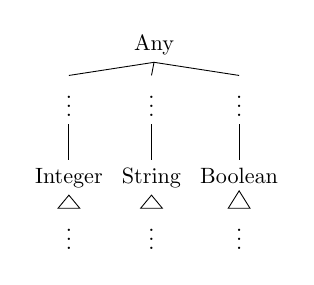
\begin{tikzpicture}[scale=.8]
            \Tree[.Any
                      [.{$\vdots$} [.Integer \edge[roof]; {$\vdots$} ] ]
                      [.{$\vdots$} [.String \edge[roof]; {$\vdots$} ] ]
                      [.{$\vdots$} [.Boolean \edge[roof]; {$\vdots$} ] ] ]
          \end{tikzpicture}
                    
          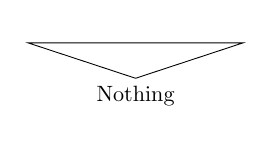
\begin{tikzpicture}[scale=.8]
            \tikzset{grow'=up}
            \Tree[.Nothing \edge[roof]; { \hspace{90pt} } ]
          \end{tikzpicture}
        \end{uncoverenv}
      \end{center}
    \end{column}

    \begin{column}{0.7\textwidth}
      \begin{itemize}
        \item<+-> どんな2つの元も、一意な共通の祖先と子孫をそれぞれ持つ
        \item<+-> 型システム理論においては、ボトム(\lstinline|Nothing|)を
        入れると複雑になると知られており避けられる傾向にあるが、Scalaには入っている
        \item<+-> そのため、Scalaのサブタイプ関係は束となる
      \end{itemize}
    \end{column}
  \end{columns}
\end{frame}

\begin{frame}[fragile]
  \frametitle{トランザクションと束}
 
  \begin{itemize}
    \item<+-> 実はトランザクションは束構造を作る
    \item<+-> そして、その束となったトランザクションを
    サブタイプで表現する
  \end{itemize}

  \begin{columns}
    \begin{column}{0.3\textwidth}
      \begin{uncoverenv}<+->
        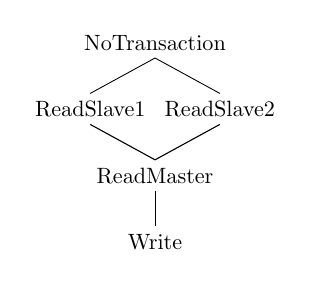
\begin{tikzpicture}[scale=.8]
          \begin{scope}
            \Tree[.NoTransaction
                          \node(s1){ReadSlave1};
                          \node(s2){ReadSlave2}; ]
          \end{scope}
                        
          \begin{scope}[yshift=-60pt]
            \Tree[.\node(r){ReadMaster}; Write ]
          \end{scope}
       
          \begin{scope}
            \draw (s1.south)--(r.north);
            \draw (s2.south)--(r.north);
          \end{scope}
        \end{tikzpicture}
      \end{uncoverenv}
    \end{column}

    \begin{column}{0.7\textwidth}
      \begin{uncoverenv}<+->
\begin{lstlisting}[style=scala]
trait NoTransaction
 
trait ReadSlave1 extends NoTransaction

trait ReadSlave2 extends NoTransaction
 
trait ReadMaster
  extends ReadSlave1 with ReadSlave2

trait Write extends ReadMaster
\end{lstlisting}
      \end{uncoverenv}
    \end{column}
  \end{columns}

  \begin{itemize}
    \item<+-> サブタイプ関係を使ってトランザクションの束構造を
    プログラム内に\textbf{型レベル}でエンコードできた
  \end{itemize}
\end{frame}
 
\begin{frame}[fragile]
  \frametitle{\Fujitask と合成}
 
  \pause
  \begin{itemize}
    \item<+-> \Fujitask の合成演算である\lstinline|flatMap|は
    次のようになっている
  \end{itemize}
    
  \begin{uncoverenv}<+->
\begin{lstlisting}[style=scala]
trait Task[-R, +A] {
  def flatMap[ER <: R, B](f: A => Task[ER, B]): Task[ER, B]
}
\end{lstlisting}
  \end{uncoverenv}
 
  \begin{itemize}
    \item<+-> これはたとえば次のようになる
    \begin{enumerate}
      \item<+-> \lstinline|Task[ReadSlave1, A]|と
      \lstinline|Task[ReadSlave1, B]|を合成したら、\lstinline|Task[ReadSlave1, B]|となる
 
      \item<+-> \lstinline|Task[ReadSlave1, A]|と
      \lstinline|Task[ReadSlave2, B]|を合成したら、\lstinline|Task[ReadMaster, B]|となる
 
      \item<+-> \lstinline|Task[ReadSlave1, A]|と
      \lstinline|Task[ReadMaster, B]|を合成したら、\lstinline|Task[ReadMaster, B]|となる
    \end{enumerate}
  \end{itemize}
\end{frame}

% \begin{frame}[fragile]
%   \frametitle{\Fujitask の実行}
%  
%   \pause
%   \begin{itemize}
%     \item<+-> \Fujitask には\lstinline|run|というメソッドがある
%   \end{itemize}
%   
%   \begin{uncoverenv}<+->
% \begin{lstlisting}[style=scala]
% trait Task[-R, +A] { lhs =>
%   def run[ER <: R]()(implicit runner: TaskRunner[ER]): Future[A]
% }
% \end{lstlisting}
%   \end{uncoverenv}
%  
%   \begin{itemize}
%     \item<+-> \lstinline|TaskRunner|は次のようにトランザクション
%     をどうするかを定義できる
%   \end{itemize}
%  
%   \begin{uncoverenv}<+->
% \begin{lstlisting}[style=scala]
% trait TaskRunner[R] {
%   def run[A](task: Task[R, A]): Future[A]
% }
% \end{lstlisting}
%   \end{uncoverenv}
% \end{frame}
%  
% \begin{frame}[fragile]
%   \frametitle{\Fujitask の実行}
%  
%   \begin{itemize}
%     \item<+-> あとは\lstinline|TaskRunner|の実装を書けばOK
%   \end{itemize}
%  
%   \begin{uncoverenv}<+->
% \begin{lstlisting}[style=scala]
% implicit val writeTaskRunner: TaskRunner[Write] =
%   new TaskRunner[Write] {
%     private val transactionManager = new TM()
%     
%     def run[A](task: Task[Write, A]): Future[A] = {
%       transactionManager.begin()
%       task.execute(new Write {})
%       transactionManager.commmit()
%     }
%   }
% \end{lstlisting}
%   \end{uncoverenv}
%  
%   \begin{itemize}
%     \item<+-> \lstinline|implicit|でトランザクションの種類を表す型に
%     もとづいた\lstinline|TaskRunner|の実装が\textbf{コンパイル時}に選択される
%   \end{itemize}
% \end{frame}

\begin{frame}[fragile]
  \frametitle{\Fujitask の実行}

  \begin{itemize}
    \item<+-> \Fujitask はモナドなので、\lstinline|for|式で
    まとめていくことができる
  \end{itemize}

  \begin{uncoverenv}<+->
\begin{lstlisting}[style=scala]
val transaction = for {
  _ <- paymentRepository.update(payment)
  _ <- userPermissionRepository.update(userPermission)
  _ <- coachRepository.assgin(coach, user)
} yield ()

transaction.run()
\end{lstlisting}
  \end{uncoverenv}

  \begin{itemize}
    \item<+-> モナド構文ですっきり書ける

    \item<+-> オブジェクト指向プログラミングのサブタイプ、
    関数型プログラミングの型クラス・モナドが美しく融合している
    \begin{itemize}
      \item サブタイプがないHaskell、モナド構文・型クラスがないJavaに\Fujitask は実装できない
    \end{itemize}
  \end{itemize}
\end{frame}


\begin{frame}
  \frametitle{ここまでのまとめ}

  \pause
  \begin{itemize}
    \item<+-> トランザクションはしばしば束構造を成す
    \item<+-> 束構造を型レベルにエンコードする手段としてサブタイプが使える
    \item<+-> 束構造に基づくアドホックな処理を、サブタイプと型クラスで実現できる
    \item<+-> オブジョクト指向プログラミングと関数型プログラミングは美しく融合されうる
  \end{itemize}
\end{frame}

\section{\Fujitask とExtensible Effects}

\begin{frame}
  \frametitle{Extensible Effects}

  \pause
  \begin{itemize}
    \item<+-> \textbf{モナド}は1つの\textbf{効果}%
    \footnote[frame]{副作用のこと。最近だと``計算効果(Computational effect)''や%
      単に``効果(Effect)''と言うこともある。}%
    を抽象化する1つの手段

    \item<+-> 1つのモナドは1つの効果しか抽象化できないため、
    \lstinline|Reader[Env, Future[Either[Err, Option[A]]]]|のような
    \emph{モナドスタック}を使って複数の効果を表現する
    \begin{itemize}
      \item<+-> しかしこうすると\lstinline|for|式で内側のモナドへアクセスしにくくなる\ce{😞}
    \end{itemize}

    \item<+-> \textbf{モナドトランスフォーマー}はこのような問題を解決するが、
    あるモナドについて専用のモナドトランスフォーマーが必要\ce{😞}

    \item<+-> \emph{Extensible Effects}は特別な仕組みなしに
    モナドスタックを表現可能\ce{😄}
  \end{itemize}
\end{frame}

\begin{frame}
  \frametitle{\Fujitask とExtensible Effects}

  \begin{itemize}
    \item<+-> \Fujitask はサブタイプが必要

    \item<+-> Extensible EffectsはHaskell生まれ、
    でもサブタイプはない!
  \end{itemize}

  \uncover<+->{
    \simplecallout{-}{blue!20}{\Fujitask をExtensible Effectsへ持っていけるか?}
  }

  \begin{itemize}
    \item<+-> ねこはる(\texttt{@halcat0x15a})さんの作った
    \href{https://github.com/halcat0x15a/kits-eff}{kits-eff}を利用
    \begin{itemize}
      \item \href{https://github.com/atnos-org/eff}{atnos-eff}とは違った
      サブタイプを利用したExtensible Effectsの実装
    \end{itemize}

    \item<+-> できたものはここ\ce{👇}\url{https://github.com/y-yu/fujitask-eff}
  \end{itemize}
\end{frame}

\begin{frame}[fragile]
  \frametitle{Example}

  \begin{itemize}
    \item<+-> こういう感じでいろいろな効果と一緒に\lstinline|for|に入れられる
  \end{itemize}

  \begin{uncoverenv}<.->
\begin{lstlisting}[style=scala]
case class User(id: Long, name: String)
// create table `user` (
//   `id` bigint not null auto_increment,
//   `name` varchar(64) not null
// )

val eff = for {
  name <- Reader.ask[String]
  user  <- userRepository.create(name)
} yield {
  logger.info(s"user is \$user")
}
Fujitask.run(Reader.run("piyo")(eff)) 
\end{lstlisting}

\begin{lstlisting}[style=plain]
ReadWriteRunner begin --------->
user is Some(User(2,piyo))
<--------- ReadWriteRunner end
\end{lstlisting}  
  \end{uncoverenv}
 
  \begin{itemize}
    \item<+-> デモ
    \item<+-> 今回はインタープリターの\lstinline|flatMap|だけ見てみましょう
  \end{itemize}
\end{frame}

\begin{frame}[fragile]
  \frametitle{\Fujitask のインタープリター}

\begin{lstlisting}[style=scala]
object Fujitask {
  def run[I <: Transaction: Manifest, A](
    eff: Eff[I, A]
  )(
    implicit runner: FujitaskRunner[I],
    ec: ExecutionContext
  ): Future[A] = {
    def handle(i: I) = new ApplicativeInterpreter[Fujitask, Any] {
      def flatMap[T, B](fa: Fujitask with Fx[T])(k: T => Eff[Any, Future[B]]): Eff[Any, Future[B]] =
        fa match {
          case Execute(f) =>
            Eff.Pure(f(ec).flatMap(a => Eff.run(k(a))))
          case _: Ask[I] =>
            k(i.asInstanceOf[T])
        }
    }
}
\end{lstlisting}

  \begin{itemize}
    \item<+-> \ce{🙄}
  \end{itemize}
\end{frame}

\begin{frame}
  \frametitle{\Fujitask のインタープリター}

  \begin{itemize}
    \item<+-> 解説しようと思ったものの、ちょっと時間がない……\ce{😇}

    \item<+-> 今回はモチベーションだけで勘弁してください\ce{🙇}

    \item<+-> 解説資料\cite{qiita_fujitask_eff}があるので
    興味がでた人はこれを読んで!

    \item<+-> あと、kits-effは\cite{shinchoku}を読むといいです
  \end{itemize}
\end{frame}

\section{まとめ}

\begin{frame}
  \frametitle{まとめ}

  \pause
  \begin{itemize}
    \item<+-> \Fujitask は関数型プログラミングとオブジェクト指向プログラミングのよい融合
  \end{itemize}
\end{frame}

\section*{参考文献}

\begin{frame}
  \frametitle{参考文献}

  \bibliographystyle{junsrt_url}
  \nocite{*}
  \bibliography{ref}
\end{frame}

\begin{frame}
  \centering
  {\Huge Thank you for your attention!}
\end{frame}

\end{document}
